\documentclass[a4paper,11pt]{book}
\usepackage{import}
\usepackage{preamb}
\makeindex

\begin{document}

\small
\begin{multicols}{3}

%\maketitle

\thispagestyle{empty}
\scriptsize
\newpage


\begin{subbox}{subbox}{}
\centering
\Large{\textbf{Network Science   \\ Cheatsheet}}
\end{subbox}

\begin{multibox}{2}
\begin{subbox}{subbox}{}
\centering

\includegraphics[width=0.8\textwidth]{pics/logo.png}
\end{subbox}
\begin{subbox}{subbox}{}
\centering
Made by \\
\large{
Remy Cazabet
}
\end{subbox}
\end{multibox}
% \section{Blocks and Community structure}


\begin{subbox}{subbox}{}
\centering
\Large{\textbf{Nodes and Edges structural indices, Centrality, node similarity}}
\end{subbox}















\begin{textbox}{Node Structural indices}

Node structural indices, often called \textit{Node centrality}, reflect how a node is characteristic of a given structural property. This is often summarized as \textit{a measure of the node importance}, however \textit{importance} and \textit{centrality} are subjective/qualitative notions. Thus a centrality, despite its name, do not necessarily measure how \textit{central} a node is, but rather how its position in the graph is typical of the property captured by this index.

\end{textbox}













\begin{textbox}{Degree Centrality}

Degree centrality is the most straighforward centrality. It can be interpreted as a measure of importance, of popularity, e.g., the more friends I have in a social network, the more \textit{important} I am in this network.

\end{textbox}





















\begin{textbox}{Farness - Closeness}
The closeness of a node measures how close a node is from all other nodes, in term of shortest paths. To interpret it, we can make a parallel with a circle: the point which has the shortest average distance to all other points of the circle is its center. The node of highest closeness is the equivalent of the center of the circle for this graph. Its formulation is easily understood as the inverse of the farness.

\noindent\rule{4cm}{0.1pt}

\textbf{Farness:} Average distance to all other nodes in the graph
\[\text{Farness}(u)=\frac{1}{N-1}\sum_{v \in V \setminus u}\ell_{u,v} \]

\textbf{Closeness:} Inverse of the farness, i.e., how close the node is to all other nodes in term of shortest paths. 
\[\text{Closeness}(u)=\frac{N-1}{\sum_{v \in V \setminus u}\ell_{u,v}} \]


\end{textbox}



\begin{textbox}{Harmonic Centrality}
\textbf{Harmonic centrality:} is a variant of the closeness defined as the average of the inverse of distance to all other nodes (Harmonic mean). Well defined on disconnected networks with $\frac{1}{\infty}=0$. Its interpretation is the same as the closeness.

\[\text{Harmonic}(u)=\frac{1}{N-1} \sum_{v \in V \setminus u} \frac{1}{\ell_{u,v}} \]

\end{textbox}

















\begin{textbox}{Clustering Coefficient}

This score (previously defined), measures the \textit{triadic closure} of a node. A high score is often interpreted as being well embedded in a particular community (friends of my friends are my friends because we all belong to the same group), a low score can be typical of a \textit{bridge} node, e.g., few connections between my friends because they belong to different social circles.
\end{textbox}
























\begin{textbox}{Centrality - Examples - 1}


\begin{figure}[H]

\begin{subfigure}{.5\textwidth}
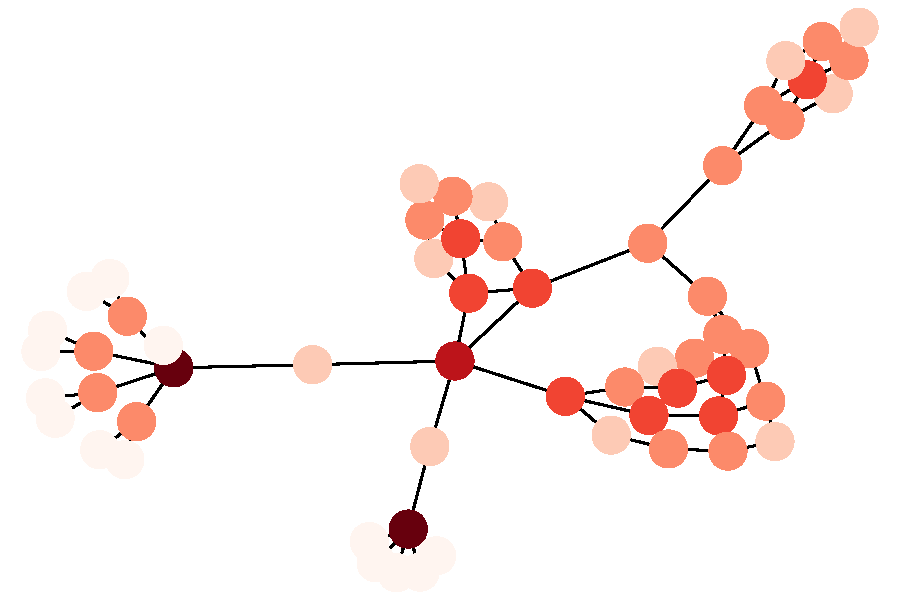
\includegraphics[width=\textwidth]{pics/exampleDegree.pdf}
    \caption{Degree}
\end{subfigure}
\begin{subfigure}{.5\textwidth}
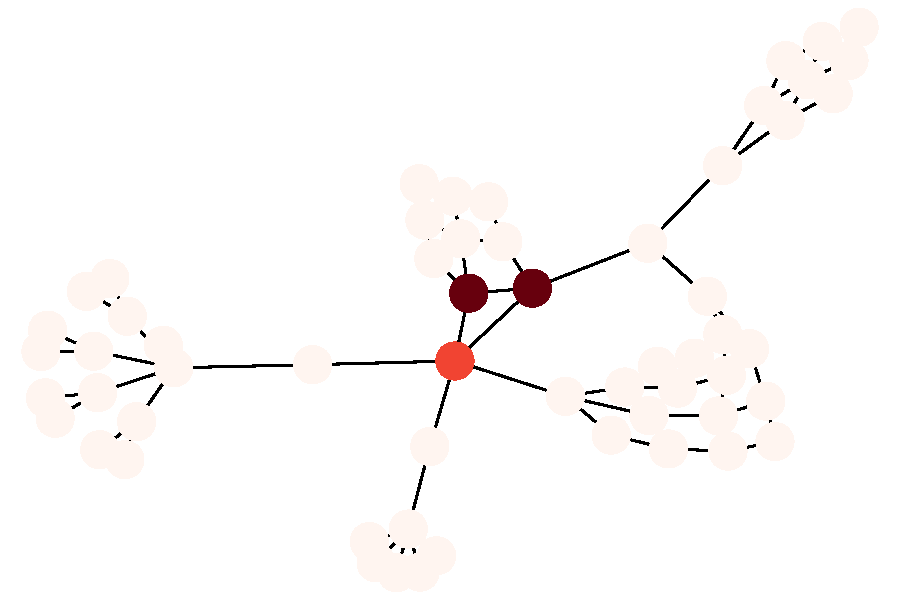
\includegraphics[width=\textwidth]{pics/exampleCC.pdf}
    \caption{Clustering Coefficent}
\end{subfigure}

\begin{subfigure}{.5\textwidth}
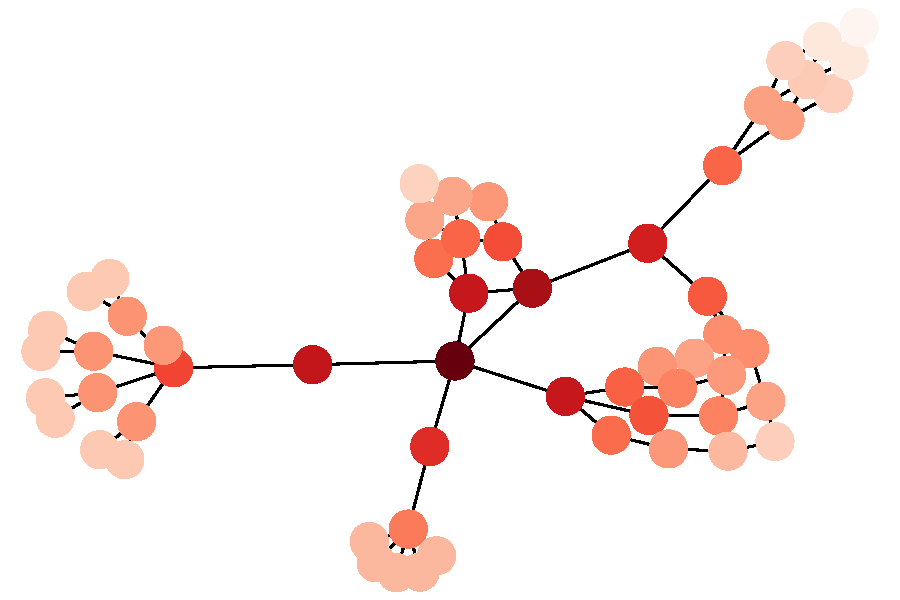
\includegraphics[width=\textwidth]{pics/exampleCloseness.pdf}
    \caption{Closeness}
\end{subfigure}
\begin{subfigure}{.5\textwidth}
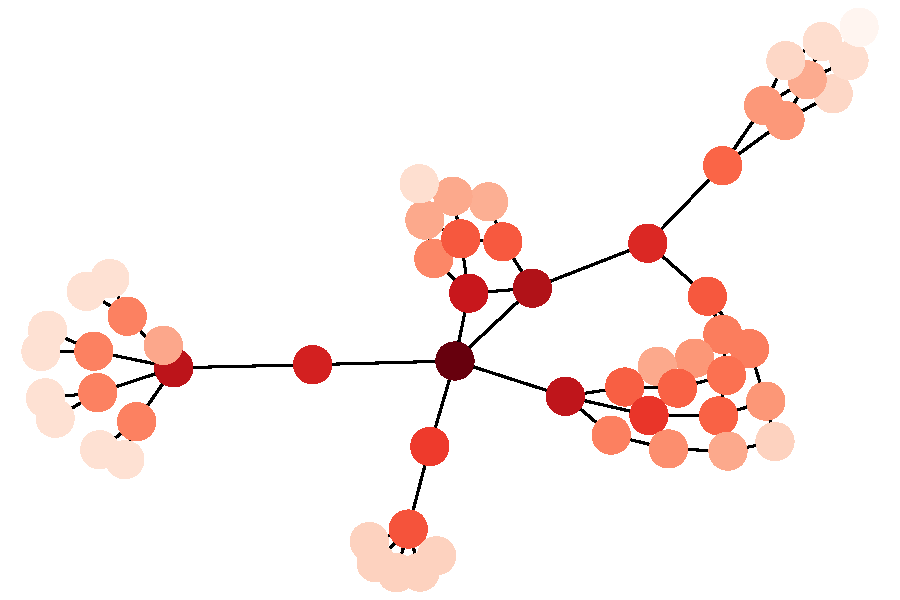
\includegraphics[width=\textwidth]{pics/exampleHarmonic.pdf}
    \caption{Harmonic Centrality}
\end{subfigure}

\end{figure}


\end{textbox}







\begin{textbox}{Centrality - Examples - 2}


\begin{figure}[H]

\begin{subfigure}{.5\textwidth}
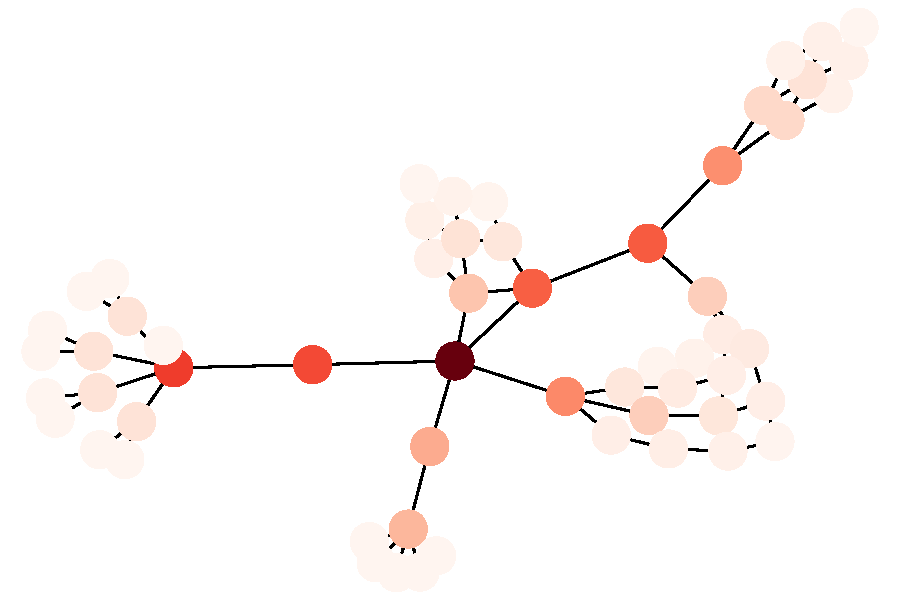
\includegraphics[width=\textwidth]{pics/examplebetweenness.pdf}
    \caption{Btwnness Centrality}
\end{subfigure}
\begin{subfigure}{.5\textwidth}
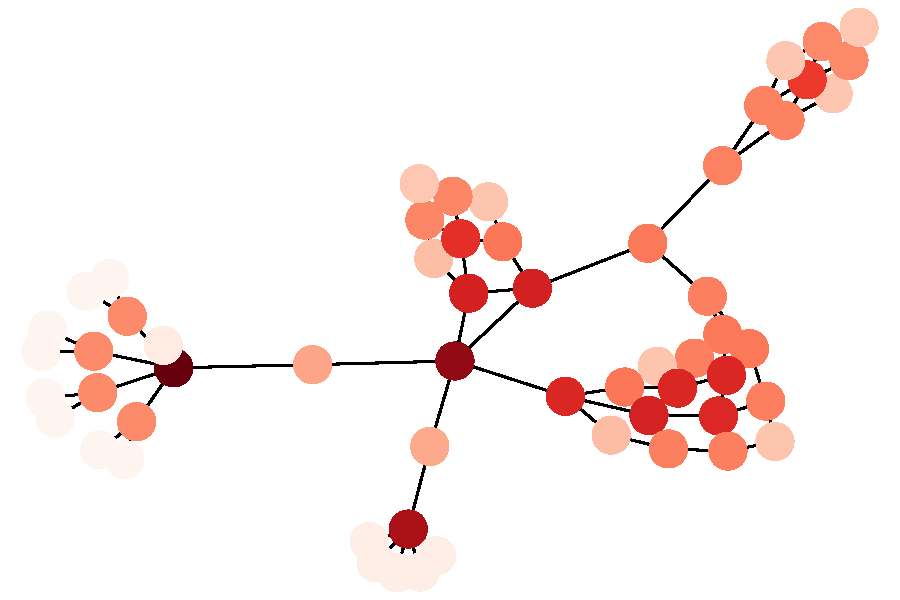
\includegraphics[width=\textwidth]{pics/exampleKatz.pdf}
    \caption{Katz Centrality}
\end{subfigure}

\begin{subfigure}{.5\textwidth}
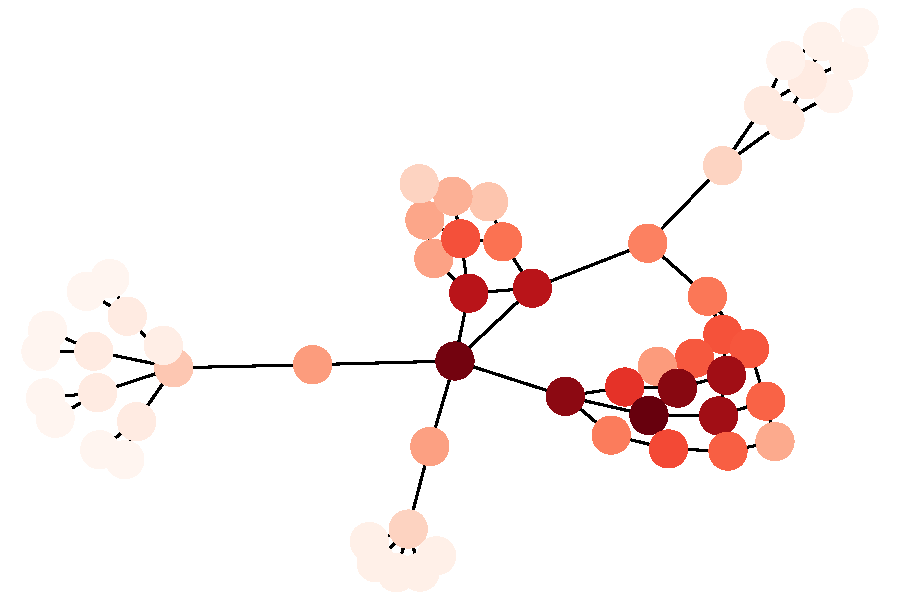
\includegraphics[width=\textwidth]{pics/exampleEigenvector.pdf}
    \caption{Eigenvector Centrality}
\end{subfigure}
\begin{subfigure}{.5\textwidth}
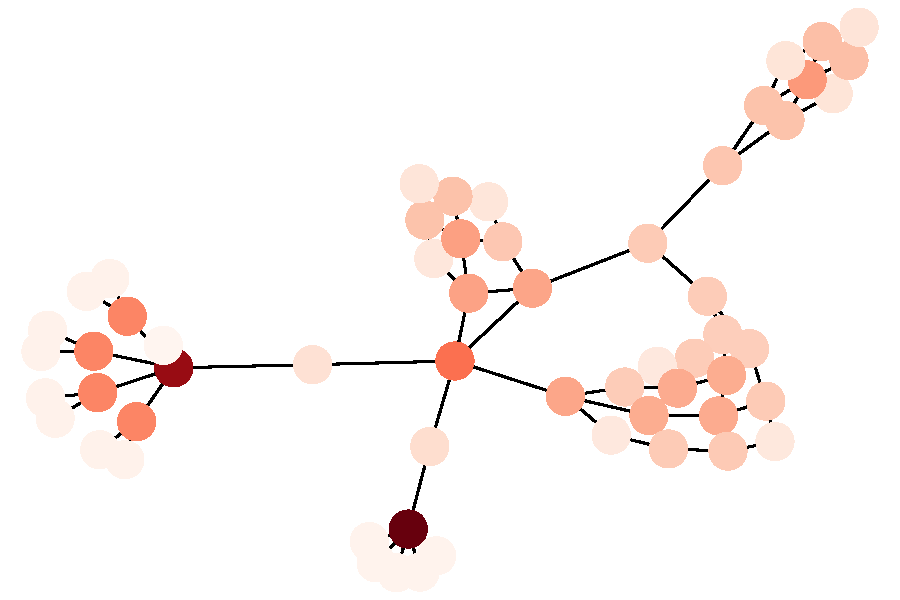
\includegraphics[width=\textwidth]{pics/examplepagerank.pdf}
    \caption{PageRank}
\end{subfigure}



\end{figure}


\end{textbox}



\begin{textbox}{Betweenness centrality}
The betweenness centrality measures how much the node plays the role of a bridge. The highest the betweenness, the more the node is essential to move quickly in the graph. More formally, the betweenness of $u$ is defined as the fraction of the shortest paths between all pairs of nodes in the graph (but $u$) that go through $u$. As a consequence, if we remove a node of high betweenness, many shortest paths will become longer, and the graph harder to navigate. The extreme situation is a node on the only path between otherwise disconnected components: if we remove this node, some nodes becomes unreachable from others. Those nodes thus tend to have high betweenness. It is defined as:

\[ C_{B}(v)=\sum _{s\neq v\neq t\in V}{\frac {\sigma _{st}(v)}{\sigma _{st}}}\]

with $\sigma _{st}$ the number of shortest paths between nodes $s$ and $t$ and $\sigma _{st}(v)$ the number of those paths passing through $v$.


The betweenness tends to grow with the network size. A normalized version can be obtained by dividing by the number of pairs of nodes, i.e., for a directed graph: $C_{B}^{\text{norm}}(v)=\frac{C_{B}(v)}{(N-1)(N-2)}$.

\end{textbox}












\begin{textbox}{Eigenvector centrality}
Eigenvector centrality is a recursive definition of importance: a node is important if it is connected to other important nodes. In practice, it is defined in the following way: the eigenvector centrality $C_u$ for every node $u$ of the graph is such that if each node \textit{sends} its centrality score to its neighbors, then the sum of scores received by each node will be equal to $\lambda C_u$ (with $\lambda$ a normalization constant). More formally,

\begin{equation}
    \centering
C^{t+1}_u = \frac{1}{\lambda}\sum_{v\in N^{in}_u}C^t_v
\label{eqpow}
\end{equation}
This recursive definition can be interpreted in term of eigenvectors and eigenvalues, which is defined as $Ax=\lambda x$, with $x$ an eigenvector, $\lambda$ the corresponding eigeinvalue. The eigenvector centrality is defined as the leading invector, i.e., the eigenvector associated with the highest eigenvalue, the only solution for which all centrality values are positive.

A simple way to compute this eigenvalue is called the power method: one starts with random values on nodes, and iterate equation \ref{eqpow}. After some time, it can be proven that the values converge to the eigenvector centrality.

\noindent\rule{4cm}{0.1pt}

Eigenvector centrality cannot in general be computed on directed networks, because of source nodes, i.e., $k^{in}=0$. Those nodes have by definition an eigenvector centrality of 0 at t+1, and thus \textit{send} a value of 0 at t+2, which might in turn result in a score of 0 for its successors, and so on and so forth.


\end{textbox}





\begin{textbox}{Katz centrality}
Katz centrality \footcite{katz1953new} is said to be a measure of the influence potential of a node. For a node $u$, it is defined as the sum, for all path length distance $\ell$, of the number of nodes located at distance exactly $\ell$ of $u$, discounted of a factor decreasing as $\ell$ increases. The intuition is that, the more nodes can be accessed in few steps, the higher the value. More formally, it is expressed as
\[
 C_{\mathrm {Katz} }(u)=\sum _{\ell=1}^{\infty }\sum _{v=1}^{N}\alpha ^{\ell}(A^{\ell})_{vu}
\]
in which $(A^{\ell})_{vu}$ means the number of paths of length $\ell$ from $v$ to $u$, and $0< \alpha < \frac{1}{\lambda_{\max}}$ an attenuation parameter smaller than the reciprocal of the largest eigenvalue of $A$, to allow computation in matrix form.
%allowing to compute with matrix form:
%\[
% C_{\mathrm {Katz} }(u)=((I- \alpha A^T)^{-1}-I)\overrightarrow{I}
%\]

\vspace{0.25cm}

Note that in a directed network, Katz centrality as presented here represents a \textit{vote} mechanism: a higher centrality of $u$ means that more nodes can reach $u$ quickly, and not that $u$ can reach many nodes quickly. We can inverse it by using $(A^{\ell})_{uv}$ instead of $(A^{\ell})_{vu}$
\end{textbox}


\begin{textbox}{Katz centrality and Eigenvector centrality}
Katz centrality can also be understood \footcite{newman2018networks} as a generalization of the eigenvector centrality, with a recursive definition, such as:
\[
C_{\mathrm {Katz} }(u) = \alpha \sum_{v\in N^{in}_u} C_{\mathrm {Katz} }(v) + \beta
\]
with $\beta=1$. We can see that with $\beta=0$ and $\alpha = 1/\lambda_{\max}$ Katz centrality is equivalent to the eigenvector centrality.

\end{textbox}





\begin{textbox}{Pagerank centrality}
Pagerank centrality is famous for being the method originally used by google to rank web-pages: all pages containing the researched words are ordered according to their Pagerank score in the graph of the WWW, in which nodes are webpages and edges are hyperlinks. 

It is a variant of the Eigenvector centrality, solving the problem of source nodes. 

Pagerank introduces two improvements: 1) at each step $t$, each node gain a small constant value. 2) The values \textit{sent} are divided equally among successors (normalization by degree). Equation \ref{eqpow} thus becomes:
\begin{equation}
    \centering
C^{t+1}_u = \alpha \sum_{v\in N^{in}_u} \frac{C^t_v}{k^{out}_v} + \beta
\end{equation}

with, by convention, $\beta=1$,$\alpha \in [0,1]$ a parameter.

Pagerank centrality can also be expressed as the leading eigenvector of the so-called \textit{Google matrix} $G$, defined as $G_{ij} = \alpha S_{ij} + (1- \alpha)/n$, with $S_{ij}$ the adjacency matrix normalized by column.

\end{textbox}





\begin{textbox}{Pagerank \& Random Walk}
Pagerank can be interpreted in term of \textbf{random walks}. If you consider a random walker moving from nodes to nodes following randomly chosen out-going links, which starts on a random node and moves an infinite number of times. Consider that at each step, this random walker can \textit{teleport} to any other node with a probability $\alpha$ instead of following an outgoing edge. Then, the probability for this random walker to be on each particular node corresponds to its Pagerank score. 

We can note that the average length of a walk before restart is $\frac{\alpha}{1-\alpha}$. The \textit{typical} value $\alpha=0.85$ thus means that random walkers move in average 5.7 times before restart, a typical value of average distance in real graphs.
\end{textbox}








\begin{textbox}{Edge Structural indices}

Edges structural positions in the network can also be described using structural properties, most of them being similar to node centralities.
\end{textbox}

\begin{textbox}{Edge Clustering}


\textbf{Edge Clustering} $C^e$ of an edge $(u,v)$ is the fraction of the neighbors of at least one of the two nodes which are neighbors of both of them, i.e.,
\[
C^e(u,v)=\frac{|N_u \cap N_v|}{|N_u \cup N_v|-2}
\]
High clustering edges are said \textit{Integrative}, low values edges are said \textit{Dispersive}.
\end{textbox}

\begin{textbox}{Edge Betweenness}


\textbf{Edge betweenness} Is defined exactly as node betweenness, but counting shortest paths going through each edge instead of each node, i.e.,
\[ C_{B}(u,v)=\sum _{s\neq t\in V}{\frac {\sigma _{st}(u,v)}{\sigma _{st}}}\]

with $\sigma _{st}$ the number of shortest paths between nodes $s$ and $t$ and $\sigma _{st}(u,v)$ the number of those paths passing through edge $(u,v)$.

\end{textbox}




















\begin{textbox}{Node Similarity}

When studying a network, one might be interested in comparing nodes between themselves, for instance to discover the most similar nodes in the network, or to assess if two nodes they are interested in share a similar network location. 

\noindent\rule{4cm}{0.1pt}

A first approach is to define the similarity between nodes $u$ and $v$, as their number of common neighbors, $\sigma_{u,v}$ as: $\sigma_{u,v}=|N_u \cap N_v|$. 


\noindent\rule{4cm}{0.1pt}

A weakness of this approach is that high degree nodes tend to be considered similar to low degree nodes.
A variant consists in normalizing by nodes degrees, thus computing the Jaccard Coefficient of neighborhoods: 
\[
\sigma_{u,v}= \frac{|N_u \cap N_v|}{|N_u \cup N_v|-2}
\]

\end{textbox}


\begin{textbox}{Cosine Similarity}

\textbf{Cosine similarity} $\sigma^{\cos}$ is a standard method to compare \textit{vectors}. It is defined for two vectors $x,y$ as :
\[
\sigma^{\cos}_{xy} = \frac{x.y}{|x||y|}
\]

This score can be used to measure the similarity between nodes neighborhoods by using as vector $x_u$ of node $u$ the row of the adjacency matrix corresponding to this node, i.e., $x_u=A_u$.

Cosine similarity of nodes then simplifies to:

\[
\sigma^{\cos}_{uv} = \frac{|N_u \cap N_v|}{\sqrt{k_u k_v}}
\]

\end{textbox}


\begin{textbox}{Pearson coefficient }

\textbf{Pearson coefficient} is a standard measure of correlation between variables $X$ and $Y$, which is defined as :
\[
r_{X,Y}=\frac{cov(X,Y)}{\sigma_X \sigma_Y}
\]
with $cov$ the covariance and $\sigma$ the standard deviation.

Much as for Cosine Similarity, we can adapt this measure to nodes similarities by considering $A$'s rows as discrete variables. The result can be understood intuitively by observing that the numerator becomes:
\[
cov(u,v)=|N_u \cap N_v|- \frac{k_u k_v}{N}
\]
which can be interpreted as the \textbf{number of common neighbors minus the expected number of common neighbors} in a randomized network, given nodes degrees.

\noindent\rule{4cm}{0.1pt}

$cov(u,v)=0$ means that the number of common neighbors is exactly what we would expect by chance given their degrees, while positive values means that they have more than expected (resp. for negative values).

\end{textbox}



\begin{textbox}{Going further}
Books on network science (see first CheatSheet) always introduce centralities.

Survey on the topic:
\begin{itemize}
    \item \cite{rodrigues2019network}
\end{itemize}
\end{textbox}




 \AtNextBibliography{\footnotesize}


\printbibliography[heading=subbibliography]


\end{multicols}



\end{document}


